\documentclass{article}
\usepackage[preprint]{neurips_2024}
\usepackage[utf8]{inputenc}
\usepackage[T1]{fontenc}
\usepackage{hyperref}
\usepackage{url}
\usepackage{booktabs}
\usepackage{amsfonts}
\usepackage{amsmath}
\usepackage{nicefrac}
\usepackage{microtype}
\usepackage{graphicx}
\usepackage{xcolor}
\usepackage{multirow}
\usepackage{subcaption}

\title{Knowledge Packs: Zero-Token Knowledge Delivery\\via KV Cache Injection}

\author{
  Andrey Pustovit\\
  Independent Researcher\\
  \texttt{andreyandreevgr@gmail.com}
}

\begin{document}

\maketitle

\begin{abstract}
Large language models require external knowledge for post-training facts, but Retrieval-Augmented Generation (RAG) consumes valuable prompt tokens. We propose \textbf{Knowledge Packs}---pre-computed key-value (KV) caches that deliver knowledge to frozen LLMs at \textbf{zero prompt token cost}. KV--prefix equivalence is a direct consequence of causal masking, yet practitioners routinely break it: we identify chat template formatting and template splitting as the primary failure modes (6--7pp degradation), explaining prior claims of KV outperforming RAG. With correct formatting, we observe \textbf{zero divergences} across 700 questions on two model families (Qwen3-8B, Llama-3.1-8B), saving up to \textbf{95\% of tokens} in multi-step accumulation. Beyond equivalence, we exploit a \textbf{RoPE asymmetry}---keys encode position, values encode content---to perform \textbf{value-space steering}: adding contrastive directions to cached values while leaving keys untouched. This creates KV states unreachable by any text, improving defensive coding scores from 0.6 to 1.9 on a 0--9 scale (Qwen3-8B; text-in-prompt achieves 3.7). Mid-layer values (33--66\%) carry the entire effect on both architectures, and independent directions compose linearly ($\cos{\approx}0$). In a \textbf{dual-channel} configuration, factual knowledge (full KV) and behavioral steering (mid-layer value deltas) operate simultaneously with zero interference at moderate steering strength. No training, no model modification.
\end{abstract}

% ============================================================
\section{Introduction}
% ============================================================

Large language models (LLMs) encode vast knowledge during pre-training, but this knowledge is static and incomplete. Retrieval-Augmented Generation \citep{lewis2020rag, guu2020realm} addresses this by inserting retrieved text into the prompt. However, each inserted fact \textbf{consumes prompt tokens}---reducing the context available for conversation, instructions, and chain-of-thought reasoning. With models increasingly used as agents that accumulate knowledge across multi-turn interactions, this token cost compounds: after 5 search steps, a RAG agent may spend 700+ tokens on retrieved facts alone.

We propose \textbf{Knowledge Packs}: pre-computed KV caches that deliver the same knowledge at zero prompt token cost. The key insight is simple: in a decoder-only transformer, causal masking ensures that prefix tokens never attend to future tokens. Therefore, the KV cache computed from a standalone forward pass on fact text $F$ is \textit{identical} to the KV entries that would be computed for $F$ during a joint forward pass on $F \circ q$ (facts concatenated with query). We formalize this as the \textbf{KV--Prefix Equivalence Property} and verify it empirically: across 500 HotpotQA questions, KV injection and text-in-prompt with identical content produce \textbf{zero divergences}.

This equivalence is the foundation, not the limitation, of our contribution. Because KV injection is provably lossless, it provides a \textbf{free optimization}: identical accuracy at reduced token cost. The savings are especially significant for knowledge-intensive agents that accumulate facts over multiple retrieval steps, where RAG's token cost grows as $O(n)$ while KV remains $O(1)$.

We further identify a critical methodological requirement: KV caches must be built using the model's chat template formatting. Raw text KV (without special tokens like \texttt{<|im\_start|>}) is out-of-distribution for instruction-tuned models, causing 6--7pp accuracy degradation. This finding explains discrepancies in prior work and is essential for correct KV injection.

Finally, we demonstrate that knowledge delivery and value steering operate as a \textbf{dual-channel architecture}: factual knowledge flows through the full KV cache while behavioral control is applied via value-space deltas on mid layers. At moderate steering strength ($\alpha{\leq}0.5$), the two channels show zero interference---opening a path to frozen LLMs that receive both \textit{what to know} and \textit{how to behave} through a single KV-space interface.

Our contributions:
\begin{enumerate}
    \item \textbf{Practical equivalence and its pitfalls.} We verify KV--prefix equivalence with zero divergences across 700 questions on two model families, and identify chat template formatting and template splitting as failure modes that explain discrepancies in prior work (6--7pp degradation from raw-text KV, 1.5pp from duplicate BOS on Llama).
    \item \textbf{Zero-token knowledge delivery at scale.} KV injection saves up to 95\% of knowledge tokens in multi-step accumulation (constant cost vs.\ RAG's linear growth). Sequential KV composition preserves positional encoding, and banked routing scales to 5{,}000+ facts.
    \item \textbf{Value-space steering via RoPE asymmetry.} Contrastive steering in value space (keys untouched) creates KV states unreachable by any text. Mid-layer values (33--66\%) carry the entire effect on both architectures, and independent directions compose linearly ($\cos{\approx}0$), enabling training-free behavior stacking.
    \item \textbf{Dual-channel architecture.} Knowledge delivery (full KV) and behavioral steering (mid-layer value deltas) operate simultaneously with zero interference at $\alpha{\leq}0.5$, demonstrating two composable control channels on a frozen LLM.
\end{enumerate}

% ============================================================
\section{Method}
% ============================================================

\subsection{KV Cache Injection}

A transformer processes input tokens through $L$ layers, each producing key and value matrices stored in the KV cache for subsequent attention. Our method pre-computes the KV cache for fact sentences \textit{offline}, then loads it as a ``virtual prefix'' at inference time.

\paragraph{Write phase (offline, once).} Given fact sentences $\{f_1, \ldots, f_n\}$, we format them using the model's chat template as a system message:

\begin{equation}
    F_{\text{chat}} = \texttt{chat\_template}(\texttt{system}: f_1 \circ \cdots \circ f_n)
\end{equation}

We tokenize $F_{\text{chat}}$ to obtain $\mathbf{x}_F = (x_1, \ldots, x_T)$ and run a forward pass:
\begin{equation}
    \text{KV}_F = \text{Model}(\mathbf{x}_F).\text{past\_key\_values}
\end{equation}
producing $(\mathbf{K}^{(l)}, \mathbf{V}^{(l)}) \in \mathbb{R}^{T \times d_k} \times \mathbb{R}^{T \times d_v}$ for each layer $l$.

\paragraph{Read phase (per query).} Given query $q$, we format it as the user message (without system message, since it is already in KV) and generate:
\begin{equation}
    \text{output} = \text{Model.generate}(\mathbf{x}_q, \; \text{past\_key\_values}=\text{KV}_F, \; \text{attention\_mask}=\mathbf{1}_{T+S})
\end{equation}

\paragraph{Chat template requirement.} A critical implementation detail: fact text \textit{must} be wrapped in the model's chat template before computing the KV cache. Instruction-tuned models expect inputs to begin with special tokens (e.g., \texttt{<|im\_start|>system} for Qwen). Raw text KV places tokens in an out-of-distribution position, causing the model to misinterpret the cached context. We measure 7pp degradation on HotpotQA and have observed catastrophic failure (0\% accuracy) on structured generation tasks.

\subsection{KV--Prefix Equivalence Property}

\begin{quote}
\textbf{Property.} For a decoder-only transformer with causal attention, let $F$ be a fact sequence and $q$ a query. Then:
$$\text{KV}(F) \oplus \text{generate}(q \mid \text{KV}(F)) \equiv \text{generate}(F \circ q)$$
That is, pre-computing KV from $F$ alone and generating $q$ with that cache produces identical output to generating from the concatenation $F \circ q$.
\end{quote}

This follows directly from causal masking: token $x_i$ attends only to positions $j \leq i$, so the KV entries for fact positions $1, \ldots, T$ are computed identically whether or not query tokens are present. A layer-by-layer induction proof is given in Appendix~\ref{app:proof}. The property holds for standard causal attention and may not hold for bidirectional or cross-attention architectures.

\subsection{Banked Routing}

For scaling beyond a single context window, we partition facts into banks via k-means clustering on BGE-large embeddings, with $B = \lceil N/20 \rceil$ banks. At query time: (1) embed query with BGE, (2) select nearest bank centroid, (3) rank facts within bank, (4) recompute KV for top fact on-the-fly (${\sim}$5\,ms). Storage: $<$1\,KB/fact (text + embedding), yielding 4\,MB for 5{,}000 facts.

\subsection{KV Composition}

Independently-built KV caches can be composed via \textbf{sequential forward passes}: process pack A to obtain $\text{KV}_A$, then process pack B \textit{with $\text{KV}_A$ as context}, producing a combined cache with continuous positional encodings. Naive concatenation (stacking caches) breaks RoPE because both start at position 0.

% ============================================================
\section{Experimental Setup}
% ============================================================

\paragraph{Models.} We evaluate on two model families to verify generality:
\begin{itemize}
    \item \textbf{Qwen3-8B} \citep{qwen3}: Primary model, fp16 on NVIDIA A100 80GB. Instruction-tuned with ChatML-style template (\texttt{<|im\_start|>}/\texttt{<|im\_end|>}).
    \item \textbf{Llama-3.1-8B-Instruct} \citep{dubey2024llama3}: Secondary model, fp16. Uses a different chat template format (\texttt{<|start\_header\_id|>}/\texttt{<|eot\_id|>}) with auto-injected system preamble (``Cutting Knowledge Date'').
\end{itemize}
Testing on two architectures with different chat templates is essential: it verifies that the equivalence theorem holds in practice across different tokenization and formatting conventions.

\paragraph{Benchmarks.}
\begin{itemize}
    \item \textbf{HotpotQA} \citep{yang2018hotpotqa}: Multi-hop QA with 2 gold + 8 distractor paragraphs per question. $N{=}500$ (Qwen) and $N{=}200$ (Llama) from the dev set (75\% bridge + 25\% comparison).
    \item \textbf{HotpotQA Accumulation}: Same question pool with 1--5 sequential retrieval steps, measuring how token cost scales. $N{=}100$ per level per model.
    \item \textbf{Value Steering}: 15 coding tasks scored for defensive patterns (0--9 scale), tested with 30 contrastive code example pairs (``good'': defensive, error-handling vs.\ ``bad'': sloppy, no checks). Both models.
    \item \textbf{Dual-Channel}: 50 HotpotQA bridge questions with simultaneous knowledge KV and formality V-delta, measuring both factual EM and behavioral effect. Qwen3-8B.
\end{itemize}

\paragraph{Methods compared.}
\begin{itemize}
    \item \textbf{Baseline}: No external knowledge.
    \item \textbf{RAG}: Retrieved paragraphs in system message via chat template.
    \item \textbf{KV-chat}: Same paragraphs as KV cache, built with chat template (same system message as RAG). \textit{This is the fair comparison}---identical text, identical formatting, different delivery mechanism.
    \item \textbf{KV-raw}: Same paragraphs as KV cache, built from raw text without chat template. Included to quantify the chat template effect.
\end{itemize}

\textbf{Critical design choice}: RAG and KV-chat use \textit{identical} system messages with identical formatting. The \textit{only} difference is whether the system message is processed as part of the prompt (RAG) or pre-computed as KV (KV-chat). This eliminates confounds from different prompt formats, different instructions, or different fact positioning that could create artificial accuracy differences.

\paragraph{Retrieval.} BGE-large-en-v1.5 \citep{xiao2023bge} top-2 retrieval from all 10 paragraphs.

\paragraph{Evaluation.} Exact match (gold answer substring in prediction) and token-overlap F1.

% ============================================================
\section{Results}
% ============================================================

\subsection{HotpotQA: KV = RAG at Zero Token Cost}

Table~\ref{tab:hotpotqa} presents our main result: with fair formatting, KV and RAG achieve identical accuracy.

\begin{table}[t]
\centering
\caption{HotpotQA results with two model families. \textbf{Fair comparison}: KV-chat and RAG use identical system messages with identical chat template formatting. The \textit{only} difference is delivery mechanism.}
\label{tab:hotpotqa}
\begin{tabular}{llccccc}
\toprule
\textbf{Model} & \textbf{Method} & \textbf{Overall} & \textbf{Bridge} & \textbf{Comp.} & \textbf{Tok.} & \textbf{Diverg.} \\
\midrule
\multirow{4}{*}{\shortstack[l]{Qwen3-8B\\($N{=}500$)}}
& Baseline & 28.4\% & 17.1\% & 62.4\% & 0 & --- \\
& RAG (BGE top-2) & 65.2\% & 60.5\% & 79.2\% & 284 & --- \\
& \textbf{KV-chat} & \textbf{65.2\%} & \textbf{60.5\%} & \textbf{79.2\%} & \textbf{0} & \textbf{0/500} \\
& KV-raw (no template) & 59.2\% & 54.1\% & 74.4\% & 0 & --- \\
\midrule
\multirow{4}{*}{\shortstack[l]{Llama-3.1-8B\\($N{=}200$)}}
& Baseline & 29.5\% & 18.7\% & 62.0\% & 0 & --- \\
& RAG (BGE top-2) & 61.5\% & 56.7\% & 76.0\% & 290 & --- \\
& \textbf{KV-chat} & \textbf{61.5\%} & \textbf{56.7\%} & \textbf{76.0\%} & \textbf{0} & \textbf{0/200} \\
& KV-raw (no template) & 56.0\% & 49.3\% & 76.0\% & 0 & --- \\
\bottomrule
\end{tabular}
\end{table}

\paragraph{Perfect equivalence across model families.} On both Qwen3-8B and Llama-3.1-8B, KV-chat and RAG produce identical results on \textit{every single question}---zero divergences across 700 total comparisons. On Qwen: 326 both correct, 0 KV-only, 0 RAG-only, 174 both wrong. On Llama: 123 both correct, 0 KV-only, 0 RAG-only, 77 both wrong. This is not approximate agreement---it is exact output equivalence, as predicted by the KV--Prefix Equivalence Property.

\paragraph{Chat template effect: $+$6--7pp.} On Qwen, KV-raw (59.2\%) vs.\ KV-chat (65.2\%) shows 6.0pp degradation; on Llama, 56.0\% vs.\ 61.5\% shows 5.5pp. The effect is concentrated on bridge questions (6.4pp on Qwen, 7.4pp on Llama) and near-zero on comparison questions. This finding explains prior claims of KV outperforming RAG: inconsistent formatting between conditions creates artificial accuracy differences.

\subsection{Accumulation Scaling: Constant vs.\ Linear Token Cost}
\label{sec:accumulation}

The key practical advantage of KV injection emerges in multi-step retrieval, where an agent accumulates facts across sequential searches (Table~\ref{tab:accumulation}).

\begin{table}[t]
\centering
\caption{Accumulation scaling ($N{=}100$ per level per model). As retrieval steps increase, RAG token cost grows linearly while KV remains constant. Accuracy is identical at every level on both models.}
\label{tab:accumulation}
\begin{tabular}{rlccccr}
\toprule
\textbf{Searches} & \textbf{Model} & \textbf{KV EM} & \textbf{RAG EM} & \textbf{KV tok} & \textbf{RAG tok} & \textbf{Savings} \\
\midrule
\multirow{2}{*}{1} & Qwen3-8B & 43.0\% & 43.0\% & 35 & 176 & 141 (80\%) \\
& Llama-3.1-8B & 42.0\% & 42.0\% & 31 & 188 & 157 (84\%) \\
\midrule
\multirow{2}{*}{2} & Qwen3-8B & 59.0\% & 59.0\% & 35 & 299 & 264 (88\%) \\
& Llama-3.1-8B & 59.0\% & 58.0\% & 31 & 305 & 274 (90\%) \\
\midrule
\multirow{2}{*}{3} & Qwen3-8B & 65.0\% & 65.0\% & 35 & 438 & 404 (92\%) \\
& Llama-3.1-8B & 61.0\% & 61.0\% & 31 & 437 & 406 (93\%) \\
\midrule
\multirow{2}{*}{5} & Qwen3-8B & 64.0\% & 64.0\% & 35 & 739 & 704 (95\%) \\
& Llama-3.1-8B & 63.0\% & 63.0\% & 31 & 724 & 693 (96\%) \\
\bottomrule
\end{tabular}
\end{table}

\begin{figure}[t]
\centering
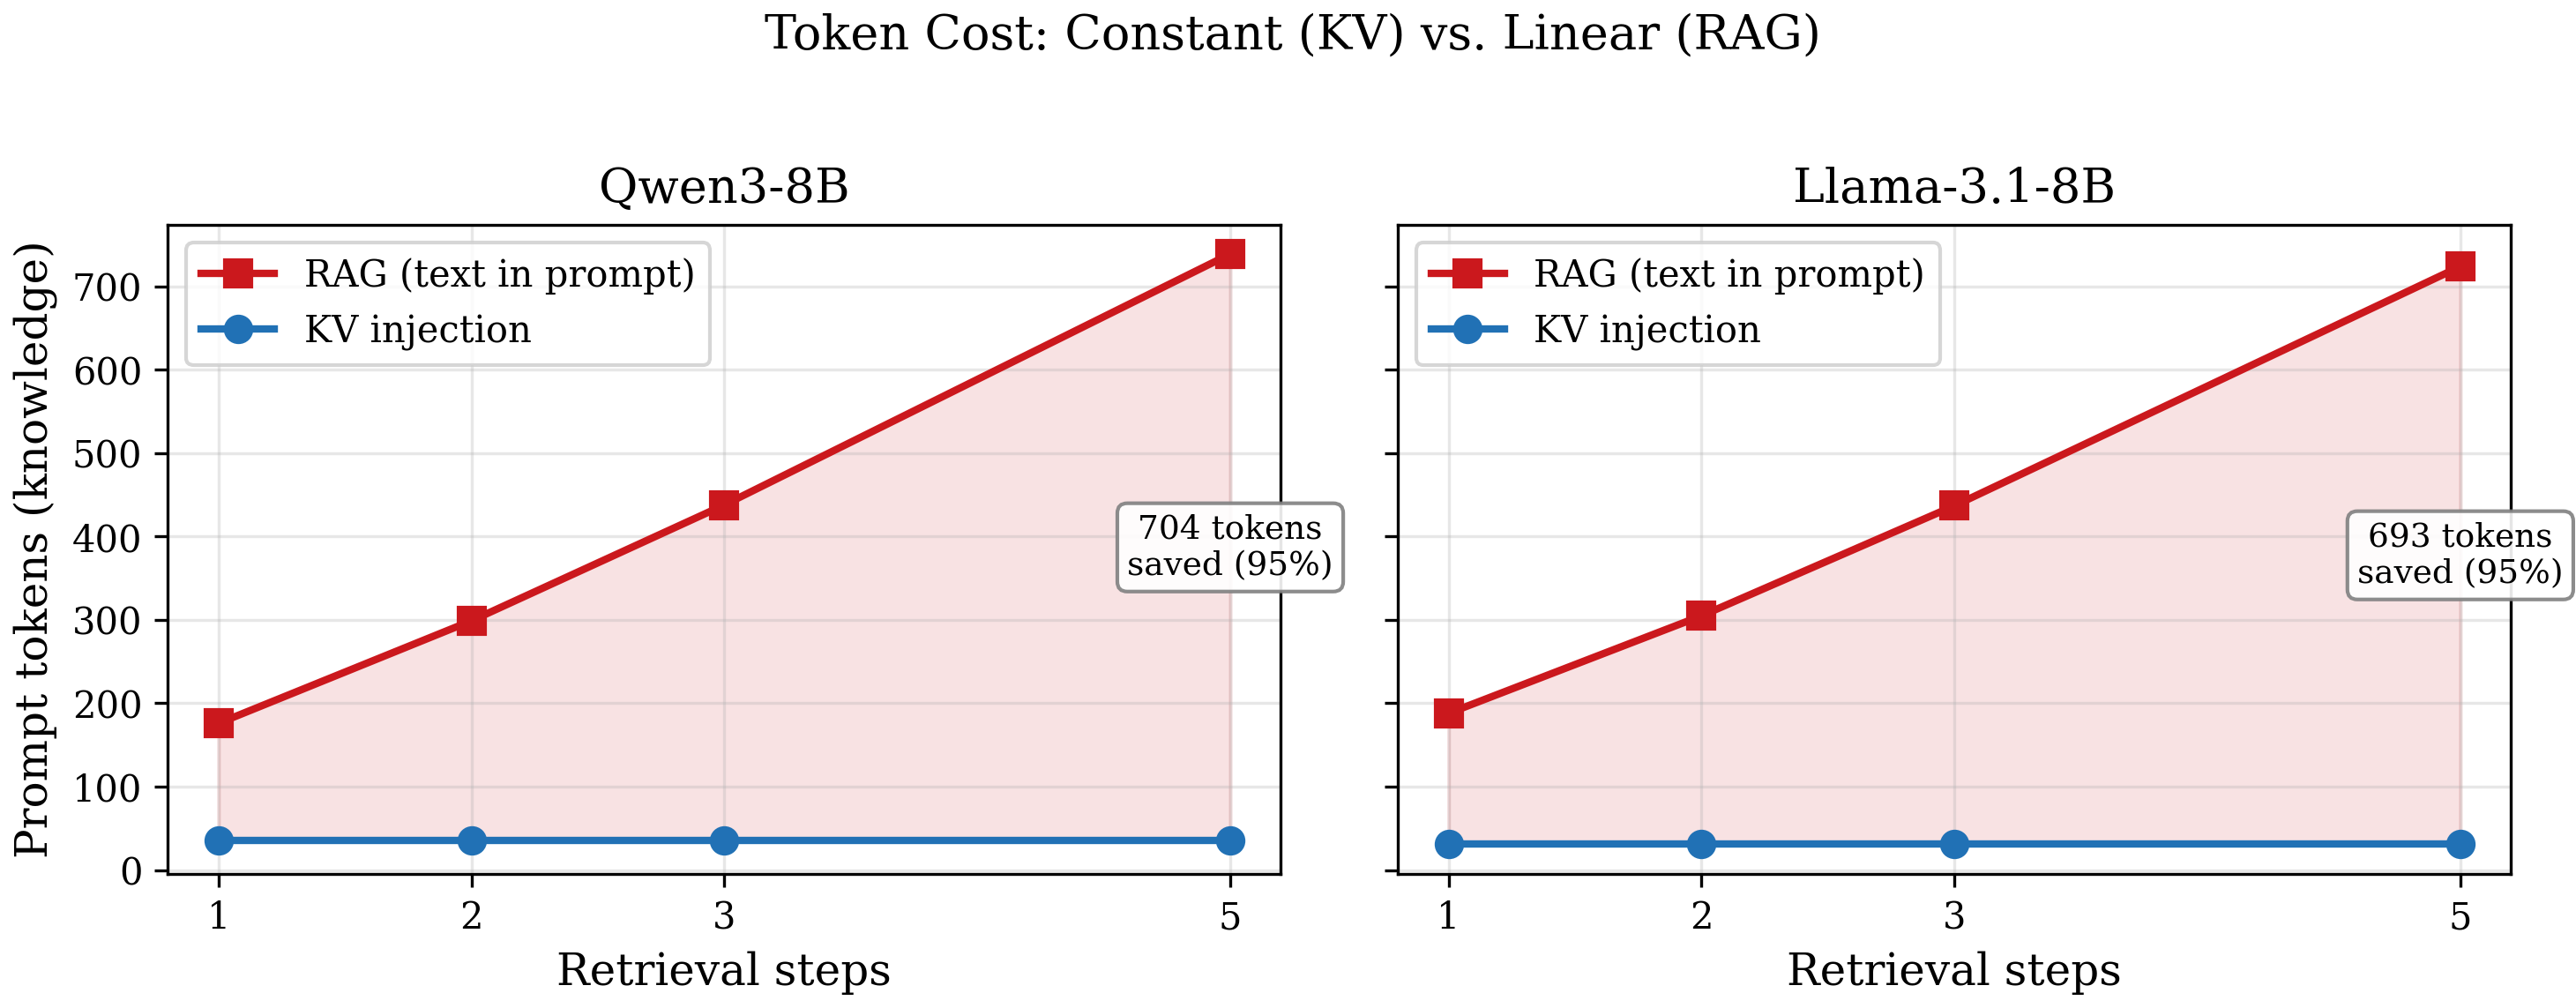
\includegraphics[width=\textwidth]{figures/accumulation_scaling.png}
\caption{Token cost scaling with retrieval steps. RAG prompt cost grows linearly (${\sim}$140--150 tokens per step) while KV injection remains constant (${\sim}$31--35 tokens). Shaded area shows cumulative token savings.}
\label{fig:accumulation}
\end{figure}

\paragraph{KV accuracy = RAG accuracy at every level, both models.} The equivalence property holds regardless of how many facts are accumulated and across both model families. The single 1pp discrepancy (Llama, 2 searches: 59\% vs.\ 58\%) is within noise for $N{=}100$. With 5 retrieval steps, both models show saturation at 3 steps, suggesting diminishing returns from additional retrieval.

\paragraph{Token savings scale linearly.} RAG token cost grows at ${\sim}$140--150 tokens per search step on both models. KV cost is constant at ${\sim}$31--35 tokens (only the user question). At 5 steps, KV saves ${\sim}$700 tokens per query---a 95--96\% reduction. For an agent processing 1{,}000 queries with 5 searches each, this saves ${\sim}$700{,}000 tokens.

\paragraph{Extrapolation.} At $k$ retrieval steps with average paragraph length $p$, RAG uses ${\sim}kp$ knowledge tokens while KV uses 0. For a 32K context window with $p{=}150$, RAG exhausts the context at ${\sim}$200 accumulated facts; KV has no such limit.

\subsection{Chat Template Analysis}
\label{sec:chat_template}

We analyze the chat template effect in detail, as it explains discrepancies between our results and prior claims of KV $>$ RAG.

\begin{table}[t]
\centering
\caption{Chat template effect by model and question type.}
\label{tab:chat_template}
\begin{tabular}{llccc}
\toprule
\textbf{Model} & \textbf{Method} & \textbf{Overall} & \textbf{Bridge} & \textbf{Comp.} \\
\midrule
\multirow{3}{*}{Qwen3-8B} & KV-chat & 65.2\% & 60.5\% & 79.2\% \\
& KV-raw & 59.2\% & 54.1\% & 74.4\% \\
& \textbf{Difference} & \textbf{+6.0pp} & \textbf{+6.4pp} & \textbf{+4.8pp} \\
\midrule
\multirow{3}{*}{Llama-3.1-8B} & KV-chat & 61.5\% & 56.7\% & 76.0\% \\
& KV-raw & 56.0\% & 49.3\% & 76.0\% \\
& \textbf{Difference} & \textbf{+5.5pp} & \textbf{+7.4pp} & \textbf{0.0pp} \\
\bottomrule
\end{tabular}
\end{table}

The chat template effect is consistent across model families (5.5--6.0pp overall) and concentrated on bridge questions. We hypothesize that raw-text KV confuses the model's ability to cross-reference multiple facts, while simpler questions are more robust to formatting noise.

\paragraph{Template split pitfall.} A second, subtler implementation issue arises when splitting the chat template between KV (system message) and prompt (user message). Na\"ively calling \texttt{apply\_chat\_template} separately for each part can introduce duplicate special tokens. On Llama-3.1, generating a user-only template re-adds \texttt{<|begin\_of\_text|>} and an empty system header, producing \texttt{system(facts) <|eot|> <|begin\_of\_text|> system() <|eot|> user(q)}---a malformed sequence that breaks equivalence (1.5pp gap in our initial experiments). The correct approach is to generate the \textit{full} template (system+user) and split it at the boundary, ensuring the concatenation is byte-identical to a single-pass template. This pitfall is model-specific: Qwen's template does not re-add BOS for user-only messages.

\paragraph{Implications for prior work.} These two pitfalls---raw-text KV and template splitting---can independently create artificial accuracy differences between KV and RAG. In combination, they can produce gaps of 5--10pp in either direction, depending on which method receives more favorable formatting. The only methodologically sound comparison uses identical formatting for both conditions, verified by checking that the concatenated KV+prompt token sequence is byte-identical to the single-pass RAG sequence.

\subsection{Scaling with Banked Routing}

We evaluate KV injection at increasing fact counts using synthetic facts with Qwen3-8B (Table~\ref{tab:scaling}).

\begin{table}[t]
\centering
\caption{Scaling KV injection with banked routing (k-means + top-1 selection + lazy recompute).}
\label{tab:scaling}
\begin{tabular}{rrccc}
\toprule
\textbf{Facts} & \textbf{Banks} & \textbf{Routing} & \textbf{Answer} & \textbf{Storage} \\
\midrule
100 & 10 & 100\% & 100\% & 0.4\,MB \\
1{,}000 & 50 & 100\% & 100\% & 1.2\,MB \\
5{,}000 & 250 & 100\% & 100\% & 4.2\,MB \\
\bottomrule
\end{tabular}
\end{table}

Routing accuracy remains 100\% across all scales. Storage grows linearly at $<$1\,KB/fact.

\subsection{KV Composition}
\label{sec:composition}

Independently-built KV caches compose via sequential forward passes with zero accuracy loss (Table~\ref{tab:composition}).

\begin{table}[t]
\centering
\caption{KV composition on HotpotQA bridge questions (Qwen3-8B, $N{=}200$). Sequential composition preserves positional encoding.}
\label{tab:composition}
\begin{tabular}{lcc}
\toprule
\textbf{Method} & \textbf{Accuracy} & \textbf{Gap vs.\ Single} \\
\midrule
KV Single (one forward pass) & 84.0\% & --- \\
KV Naive (concat, broken positions) & 78.0\% & $-$6.0pp \\
\textbf{KV Sequential (correct positions)} & \textbf{84.5\%} & \textbf{+0.5pp} \\
\bottomrule
\end{tabular}
\end{table}

Naive concatenation degrades by 6pp due to duplicated RoPE positions. Sequential composition avoids this entirely, enabling modular knowledge packs.

% ============================================================
\subsection{Beyond Equivalence: Value-Space Steering}
\label{sec:steering}
% ============================================================

The Equivalence Property establishes that KV injection \textit{reproduces} text. But can KV operations create model states \textit{unreachable by any text}? We investigate \textbf{contrastive value steering}: given ``good'' and ``bad'' example KV caches built from matched code pairs, we extract a steering direction in value space and apply it to a fresh base cache.

\paragraph{Why values, not keys.} In RoPE-based architectures \citep{su2024roformer}, key vectors encode positional information via rotation: $\mathbf{k}_i = R_{\theta}(i) \cdot W_K \mathbf{x}_i$. Arithmetic on rotated keys (blending, averaging, subtracting) produces vectors at incoherent positions, destroying the attention routing mechanism. We confirm this empirically: full-KV arithmetic (both K and V) yields incoherent output (27\% coherence at $\alpha{=}1.0$). Value vectors, in contrast, carry semantic content \textit{without} positional encoding: $\mathbf{v}_i = W_V \mathbf{x}_i$. This asymmetry is the key insight: we can perform arithmetic in value space while preserving the attention routing in key space.

\paragraph{Method.} We construct matched contrastive pairs of code examples: ``good'' (defensive, with error handling, type checks, edge cases) and ``bad'' (sloppy, with common pitfalls). Both share identical structure and variable names, differing only in quality. We build KV caches $\text{KV}_{\text{good}}$ and $\text{KV}_{\text{bad}}$ from these corpora, then steer a fresh base cache:
\begin{equation}
    \mathbf{V}^{(l)}_{\text{steered}} = \mathbf{V}^{(l)}_{\text{base}} + \alpha \cdot (\mathbf{V}^{(l)}_{\text{good}} - \mathbf{V}^{(l)}_{\text{bad}}), \quad \mathbf{K}^{(l)}_{\text{steered}} = \mathbf{K}^{(l)}_{\text{base}}
\end{equation}
Keys are \textit{never modified}, preserving attention routing. This is analogous to activation steering \citep{turner2023activation, li2024inference}, but operates on cached values rather than hidden states---enabling steering without re-running inference.

\paragraph{Alpha sweep.} Table~\ref{tab:alpha} shows the effect of steering strength $\alpha$ on both model families. Score measures defensive coding quality (0--9 scale, 15 tasks, pattern matching); coherence is the fraction of syntactically valid outputs.

\begin{table}[t]
\centering
\caption{Value steering alpha sweep with 30 contrastive pairs on two models. Optimal $\alpha$ and coherence cliff differ, but both models show significant improvement over baseline at 100\% coherence.}
\label{tab:alpha}
\begin{tabular}{rcccccc}
\toprule
 & \multicolumn{3}{c}{\textbf{Qwen3-8B} (36L)} & \multicolumn{3}{c}{\textbf{Llama-3.1-8B} (32L)} \\
\cmidrule(lr){2-4} \cmidrule(lr){5-7}
$\alpha$ & Score & Coh. & & Score & Coh. & \\
\midrule
0.0 & 0.60 & 100\% & & 1.47 & 100\% & \\
0.5 & 0.87 & 100\% & & 1.87 & 100\% & \\
1.0 & 1.13 & 100\% & & 2.00 & 100\% & \\
\textbf{1.5} & 1.60 & 100\% & & \textbf{2.47} & \textbf{100\%} & \textbf{+68\%} \\
\textbf{2.0} & \textbf{1.93} & \textbf{100\%} & \textbf{+222\%} & 2.33 & 100\% & \\
3.0 & 0.40 & 20\% & & 1.93 & 100\% & \\
5.0 & 0.00 & 27\% & & 1.33 & 93\% & \\
7.0 & 0.00 & 0\% & & 0.20 & 27\% & \\
\midrule
\multicolumn{4}{l}{\textit{Text-in-prompt}: 3.67} & \multicolumn{3}{l}{\textit{Text-in-prompt}: 3.80} \\
\bottomrule
\end{tabular}
\end{table}

Both models show monotonic improvement with $\alpha$ up to a model-specific optimum: $\alpha{=}2.0$ for Qwen (0.60$\to$1.93) and $\alpha{=}1.5$ for Llama (1.47$\to$2.47). In absolute terms, these remain well below text-in-prompt baselines (3.67 and 3.80 respectively), indicating that value-space steering nudges rather than replaces explicit instructions. The coherence cliff differs: Qwen collapses sharply at $\alpha{=}3.0$ (20\% coherence), while Llama degrades gradually (still 100\% at $\alpha{=}3.0$, 93\% at $\alpha{=}5.0$). Both models maintain 100\% coherence at their optimal $\alpha$ while using \textbf{zero prompt tokens}.

\paragraph{Layer-selective steering.} We apply value steering to layer subsets on both models (Table~\ref{tab:layers}).

\begin{table}[t]
\centering
\caption{Layer-selective value steering on two models (each at its optimal $\alpha$, 30 pairs). Mid layers (33--66\%) carry the steering effect on both architectures.}
\label{tab:layers}
\begin{tabular}{lccccc}
\toprule
 & \multicolumn{2}{c}{\textbf{Qwen3-8B} ($\alpha{=}2.0$)} & \multicolumn{2}{c}{\textbf{Llama-3.1-8B} ($\alpha{=}1.5$)} \\
\cmidrule(lr){2-3} \cmidrule(lr){4-5}
\textbf{Layer Range} & $n$ & Score & $n$ & Score \\
\midrule
All (0--100\%) & 36 & 1.93 & 32 & 2.47 \\
Early (0--33\%) & 11 & 1.20 & 10 & 1.33 \\
\textbf{Mid (33--66\%)} & \textbf{12} & \textbf{1.93} & \textbf{11} & \textbf{2.27} \\
Late (66--100\%) & 13 & 0.67 & 11 & 1.47 \\
\midrule
Baseline & --- & 0.60 & --- & 1.47 \\
\bottomrule
\end{tabular}
\end{table}

\begin{figure}[t]
\centering
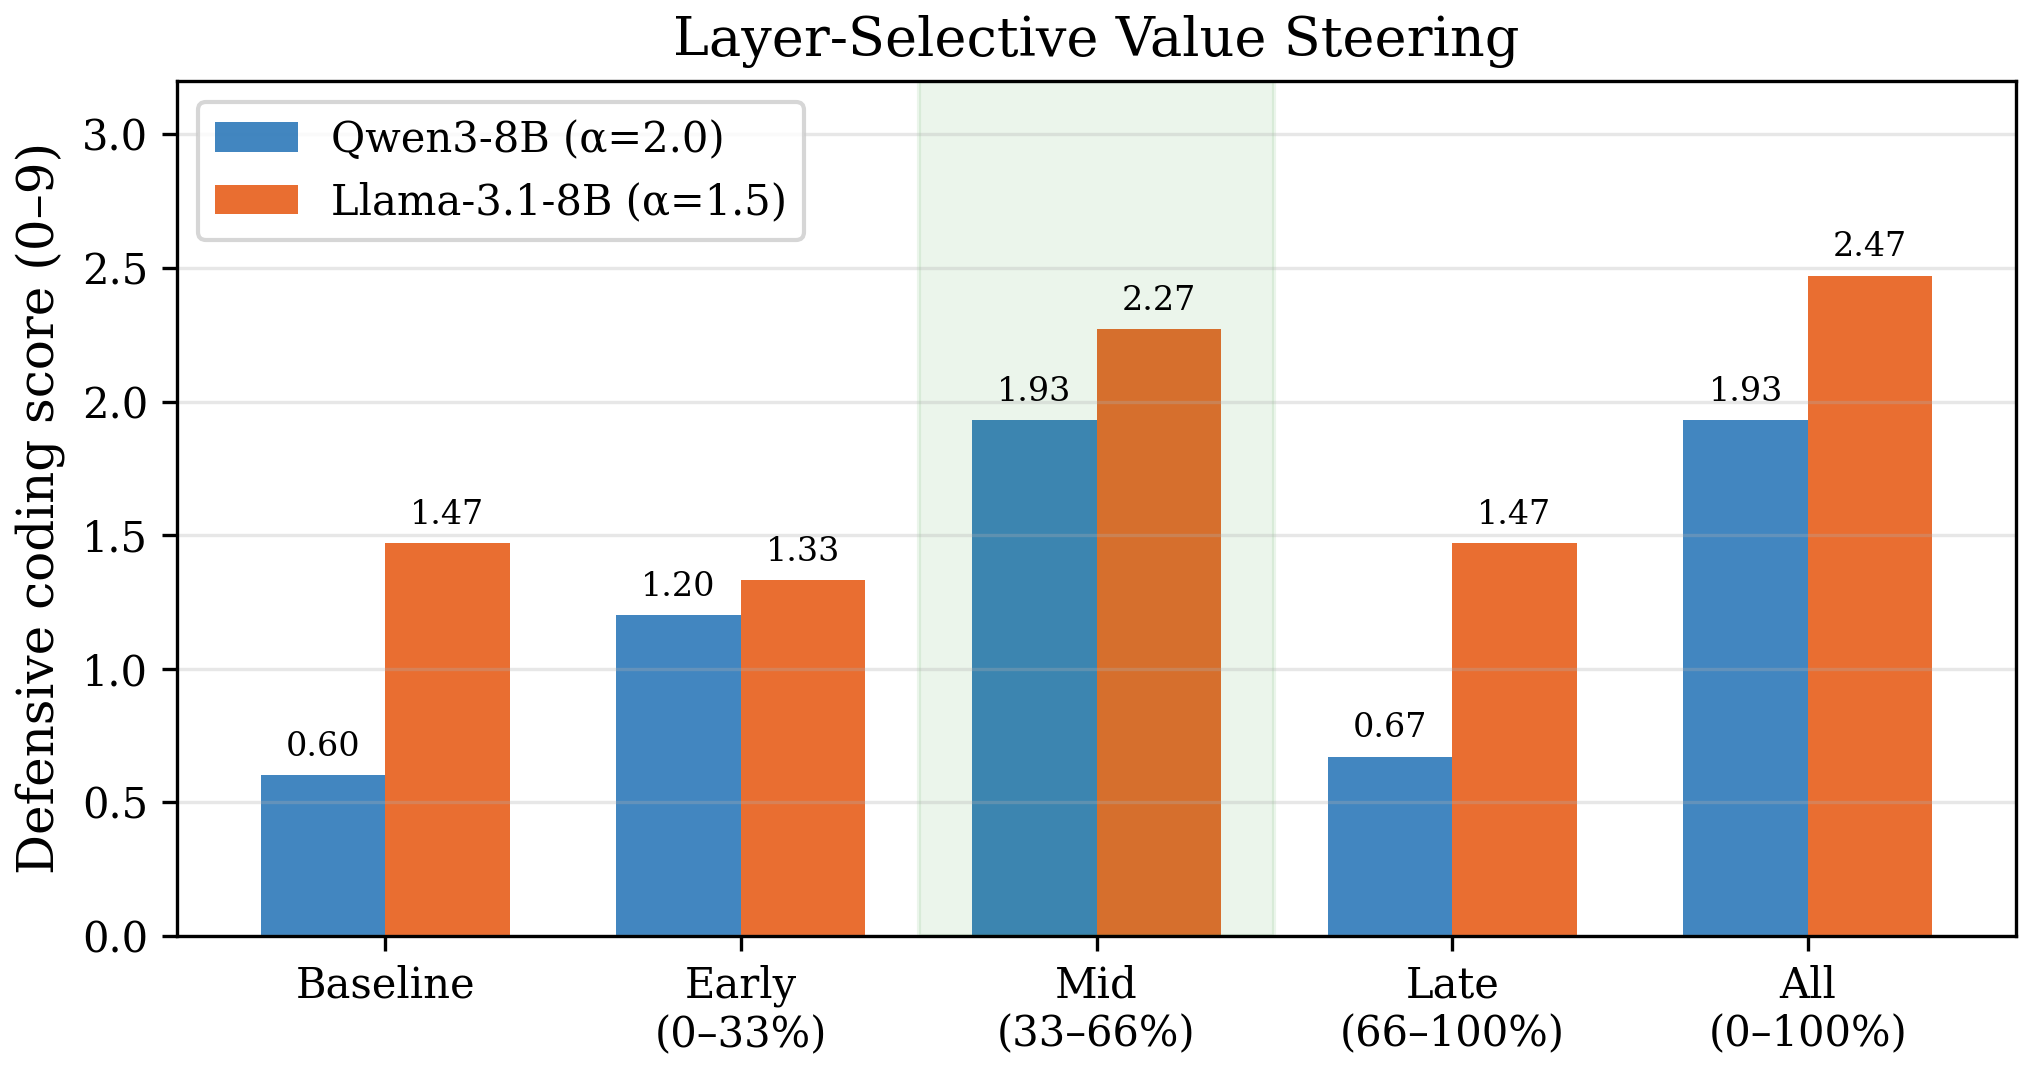
\includegraphics[width=0.7\textwidth]{figures/layer_steering.png}
\caption{Layer-selective value steering on two models. Mid layers (33--66\%, green highlight) capture the full steering effect, matching all-layer steering. Late layers produce scores indistinguishable from baseline.}
\label{fig:layers}
\end{figure}

The mid-layer result reproduces across architectures: on Qwen, mid layers (33--66\%) capture 100\% of the steering effect (1.93 = all layers); on Llama, mid layers capture 92\% (2.27 vs.\ 2.47). On both models, late layers produce scores indistinguishable from baseline (0.67 vs.\ 0.60 on Qwen; 1.47 vs.\ 1.47 on Llama). This cross-model consistency suggests that semantic style is encoded in mid-layer value representations as a general property of RoPE transformers, not an artifact of one architecture.

\paragraph{Corpus scaling.} Increasing the contrastive corpus from 5 to 30 pairs does not improve steering (1.13 at all sizes, $\alpha{=}1.0$), indicating that the steering direction saturates with minimal examples. Meanwhile, text-in-prompt quality \textit{decreases} with more examples (4.13 $\to$ 3.67), likely due to context noise.

\paragraph{Composable steering.} If individual V-deltas are approximately orthogonal, multiple can be applied simultaneously (Table~\ref{tab:compose}):
\begin{equation}
    \mathbf{V}_{\text{steered}} = \mathbf{V}_{\text{base}} + \sum_{i} \alpha_i \cdot \Delta \mathbf{V}_i, \quad \mathbf{K}_{\text{steered}} = \mathbf{K}_{\text{base}}
\end{equation}

We test two orthogonal directions: ``defensive coding'' ($\Delta \mathbf{V}_A$: error handling, type checks) and ``documentation'' ($\Delta \mathbf{V}_B$: docstrings, type hints, comments). The cosine similarity between these deltas is $0.0003 \pm 0.012$---near-perfectly orthogonal.

\begin{table}[t]
\centering
\caption{Composable value steering on two models. ``Def.'' counts error-handling patterns (0--9), ``Doc.'' counts docstring/type-hint patterns (0--11). Retention shows A+B score as percentage of single-direction score.}
\label{tab:compose}
\begin{tabular}{lcccccc}
\toprule
 & \multicolumn{3}{c}{\textbf{Qwen3-8B} ($\alpha{=}2.0$)} & \multicolumn{3}{c}{\textbf{Llama-3.1-8B} ($\alpha{=}1.5$)} \\
\cmidrule(lr){2-4} \cmidrule(lr){5-7}
\textbf{Condition} & Def. & Doc. & Coh. & Def. & Doc. & Coh. \\
\midrule
Baseline & 0.40 & 0.00 & 100\% & 1.47 & --- & 100\% \\
\midrule
$A$ only (defensive) & 1.27 & 1.00 & 100\% & 1.87 & 3.80 & 100\% \\
$B$ only (documented) & 0.73 & 3.80 & 100\% & 1.93 & 3.53 & 100\% \\
\textbf{$A{+}B$ composed} & \textbf{1.67} & \textbf{3.40} & \textbf{100\%} & \textbf{2.13} & \textbf{4.07} & \textbf{100\%} \\
\midrule
Def.\ retention & \multicolumn{3}{c}{131\%} & \multicolumn{3}{c}{114\%} \\
Doc.\ retention & \multicolumn{3}{c}{89\%} & \multicolumn{3}{c}{115\%} \\
\midrule
$\cos(\Delta V_A, \Delta V_B)$ & \multicolumn{3}{c}{0.0003} & \multicolumn{3}{c}{0.040} \\
\bottomrule
\end{tabular}
\end{table}

Composability reproduces across models: on Qwen, A+B retains 131\%/89\% of individual defensive/documentation scores; on Llama, 114\%/115\%---both showing constructive interference where composing two directions \textit{improves} over individual steering. The contrastive deltas are near-orthogonal on both models ($\cos{=}0.0003$ on Qwen, $\cos{=}0.040$ on Llama), consistent with independent encoding of behavioral properties in value space. This is analogous to LoRA stacking, but operates at inference time with no training: pre-compute two contrastive deltas offline, compose them with a single vector addition.

\paragraph{Significance.} Value steering creates KV states that have \textbf{no textual equivalent}: there is no string one could prepend to the prompt that would produce the same KV cache as $\mathbf{V}_{\text{base}} + \sum_i \alpha_i \cdot \Delta \mathbf{V}_i$. This breaks the Equivalence Property in a controlled way, opening a design space beyond text-reproducible states. The cross-model consistency of all three findings---mid-layer localization, composability with constructive interference, and near-orthogonal deltas---suggests that the value space supports a modular ``behavior algebra'' as a general property of RoPE transformers. The approach requires no training, no gradient computation, and adds zero prompt tokens---only a one-time offline computation of contrastive KV caches.

\subsection{Dual-Channel Architecture: Knowledge + Steering}
\label{sec:dual}

The preceding sections establish two independent capabilities: lossless knowledge delivery (Section~\ref{sec:accumulation}) and behavioral steering (Section~\ref{sec:steering}). The key architectural question is whether they \textbf{compose}: can a model simultaneously receive factual knowledge through full KV and behavioral control through value-space deltas?

We test this on 50 HotpotQA bridge questions (Qwen3-8B), measuring both factual accuracy (exact match on gold answers) and behavioral effect (response verbosity and formality). The knowledge channel uses gold paragraphs in a KV cache (same as Section~\ref{sec:accumulation}); the steering channel applies a ``formal/detailed'' V-delta to mid layers (33--66\%). We evaluate six conditions (Table~\ref{tab:dual}).

\begin{table}[t]
\centering
\caption{Dual-channel experiment: knowledge delivery + value steering simultaneously (Qwen3-8B, $N{=}50$ HotpotQA bridge questions). EM = exact match, Form. = formality score, Words = average response length.}
\label{tab:dual}
\begin{tabular}{llccc}
\toprule
& \textbf{Condition} & \textbf{EM} & \textbf{Form.} & \textbf{Words} \\
\midrule
A & No knowledge, no steering & 16.0\% & 0.02 & 33 \\
B & Knowledge only (KV) & 84.0\% & 0.18 & 34 \\
C & Steering only (V-delta) & 18.0\% & 0.08 & 186 \\
D & \textbf{Knowledge + Steering ($\alpha{=}2.0$)} & 64.0\% & 0.26 & 191 \\
E & Text knowledge (RAG) & 84.0\% & 0.18 & 34 \\
F & Text knowledge + text steering & 84.0\% & 0.28 & 147 \\
\bottomrule
\end{tabular}
\end{table}

At $\alpha{=}2.0$ (optimal for steering-only tasks), the knowledge channel degrades by 20pp (84\%$\to$64\% EM). The steering effect is present (words increase 6$\times$) but too aggressive. This motivates an $\alpha$ sweep for the dual-mode regime (Table~\ref{tab:dual_alpha}).

\begin{table}[t]
\centering
\caption{Alpha sweep for dual mode (knowledge + steering). At $\alpha{\leq}0.5$, factual accuracy is fully preserved while steering effect is measurable. The Pareto frontier is governed by a single scalar.}
\label{tab:dual_alpha}
\begin{tabular}{rccc}
\toprule
$\alpha$ & \textbf{EM} & \textbf{Formality} & \textbf{Words} \\
\midrule
0.0 & 84.0\% & 0.18 & 34 \\
0.1 & 84.0\% & 0.18 & 36 \\
0.2 & 84.0\% & 0.18 & 37 \\
\textbf{0.5} & \textbf{84.0\%} & \textbf{0.24} & \textbf{50} \\
0.7 & 82.0\% & 0.26 & 63 \\
1.0 & 80.0\% & 0.28 & 83 \\
1.5 & 74.0\% & 0.28 & 148 \\
2.0 & 64.0\% & 0.26 & 191 \\
\bottomrule
\end{tabular}
\end{table}

\begin{figure}[t]
\centering
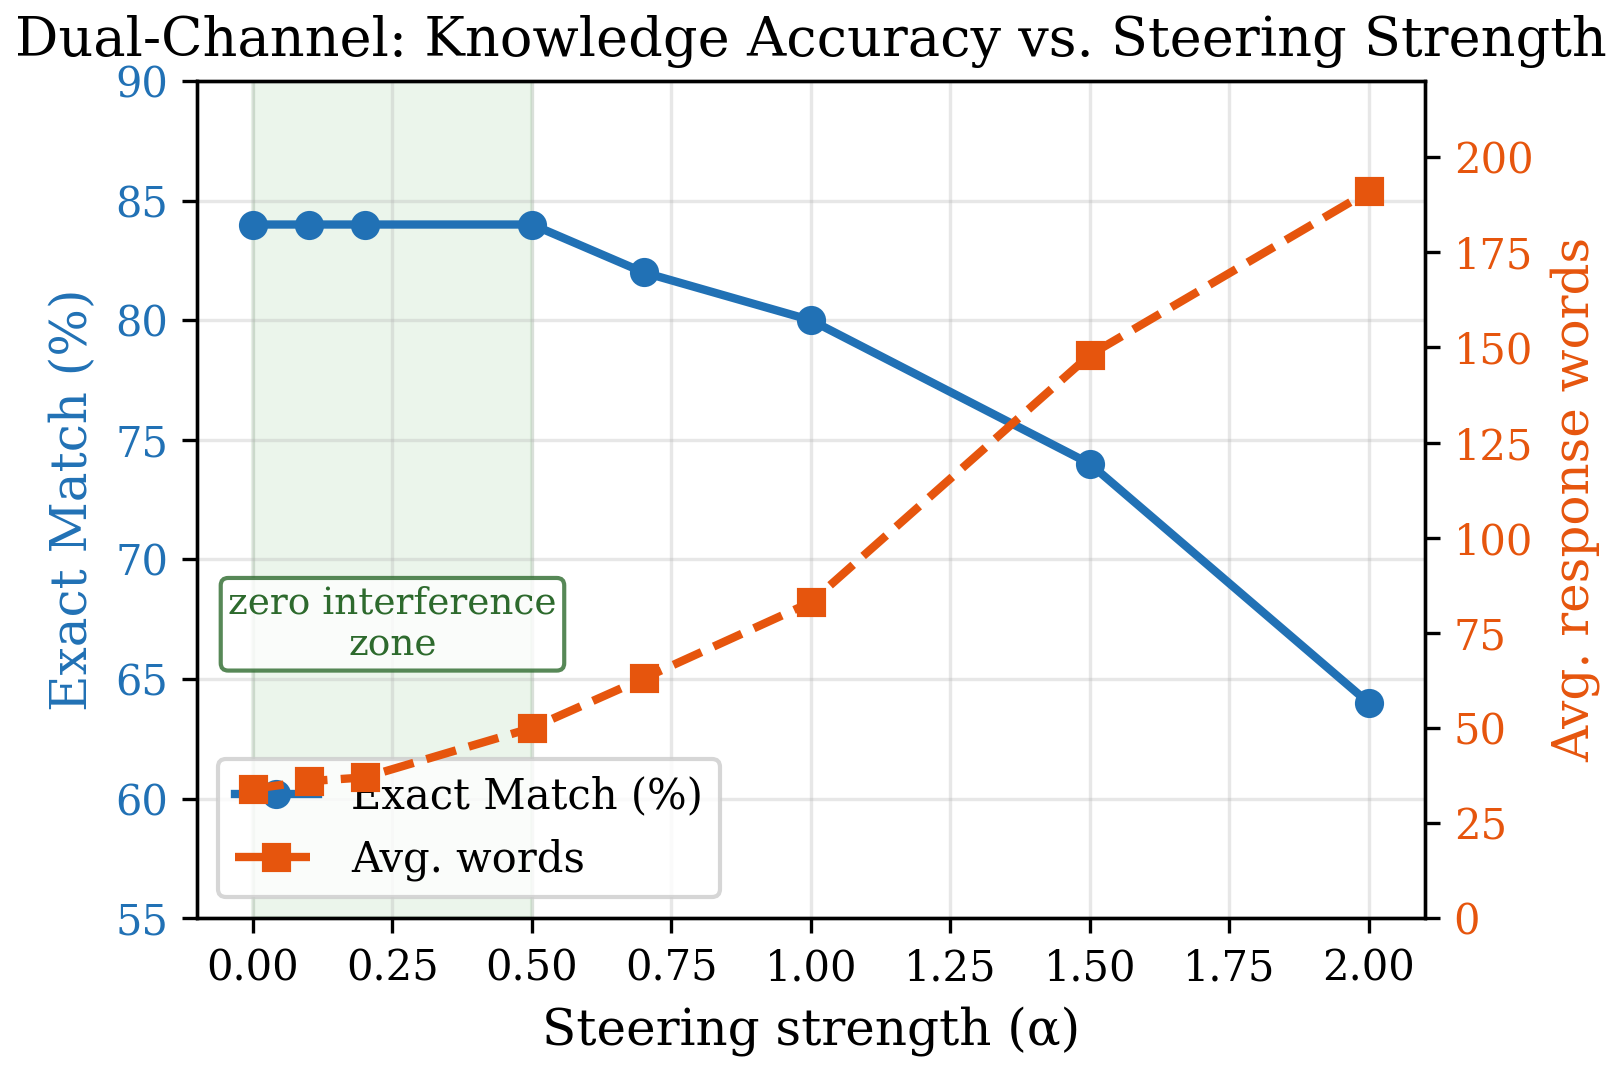
\includegraphics[width=0.65\textwidth]{figures/dual_channel_alpha.png}
\caption{Dual-channel trade-off (Qwen3-8B, $N{=}50$). At $\alpha{\leq}0.5$ (green zone), factual accuracy is fully preserved while behavioral steering is measurable. Higher $\alpha$ trades accuracy for stronger steering.}
\label{fig:dual_alpha}
\end{figure}

\paragraph{Zero-interference regime.} At $\alpha{=}0.5$, factual accuracy is \textbf{identical} to the knowledge-only baseline (84.0\% = 84.0\%) while the steering effect is measurable: formality increases by 33\% (0.18$\to$0.24) and response length by 47\% (34$\to$50 words). The two channels operate without interference through the same KV cache, using zero prompt tokens for both knowledge and behavior.

\paragraph{Pareto frontier.} The $\alpha$ parameter governs a smooth trade-off between knowledge preservation and steering strength. At $\alpha{\leq}0.5$: zero knowledge loss. At $\alpha{=}0.7{-}1.0$: mild degradation ($-$2--4pp) with stronger behavioral effect. At $\alpha{\geq}1.5$: steering dominates and factual accuracy degrades significantly. This single-scalar control enables practitioners to choose their operating point.

\paragraph{Architectural interpretation.} The dual-channel result completes the Knowledge Pack architecture. Knowledge is delivered through the \textit{full} KV cache (all layers, both keys and values)---this is the Equivalence Property channel. Behavior is steered through \textit{value deltas on mid layers only} (33--66\%, keys untouched)---this is the value-steering channel. The two channels are partially orthogonal: knowledge is distributed across all layers and both K/V, while steering operates on a subset of layers and only on V. At moderate $\alpha$, the mid-layer value perturbation is small enough not to corrupt the factual information encoded in the same positions.

% ============================================================
\section{Analysis and Discussion}
% ============================================================

\paragraph{Why equivalence matters.} The KV--Prefix Equivalence Property may seem like a negative result (``KV doesn't beat RAG''), but we argue it is the strongest possible foundation for KV injection as a practical tool. Equivalence means KV is a \textbf{lossless compression} of prompt-based knowledge delivery. Users can replace RAG text with KV caches and be \textit{guaranteed} identical outputs. No accuracy trade-off, no hyperparameter tuning, no risk of degradation.

\paragraph{When token savings matter most.}
\begin{itemize}
    \item \textbf{Pay-per-token APIs}: Prompt tokens are billed. KV injection eliminates knowledge token costs entirely.
    \item \textbf{Long conversations}: In multi-turn dialogue, accumulated RAG context competes with conversation history for the finite context window. KV frees this space.
    \item \textbf{Agentic workflows}: Agents that search, remember, and reason across many steps accumulate facts linearly. KV keeps the prompt lean.
    \item \textbf{Latency}: While KV build has overhead (${\sim}$5ms per fact), this is amortized across queries. For repeated-use knowledge (e.g., user profiles, domain facts), the amortization is substantial.
\end{itemize}

\paragraph{Same-model constraint.} KV caches are model-specific: the key/value projections differ between architectures. A KV cache from Llama cannot be loaded into Qwen. This is the primary limitation compared to RAG, which is model-agnostic.

\paragraph{Chat template as distribution shift.} The 6--7pp degradation from raw-text KV reveals that instruction-tuned models have strong expectations about token distribution at the start of input. Special tokens (\texttt{<|im\_start|>}, \texttt{<|begin\_of\_text|>}) act as ``mode switches'' that prepare the model for instruction following. Raw text before these tokens is out-of-distribution, causing the model to misinterpret the KV context. This effect is consistent across Qwen and Llama families despite their different template formats, suggesting it is a general property of instruction tuning.

\paragraph{Correcting prior claims.} Some prior work reports KV injection outperforming RAG by 5--15pp. We identify three formatting confounds that produce such artifacts: (1)~raw-text KV without chat template ($-$6pp), (2)~duplicate BOS from na\"ive template splitting ($-$1.5pp on Llama), and (3)~different system prompts or fact positioning between conditions (variable). When all confounds are eliminated, the advantage is exactly 0pp across 700 questions and two model families---as the equivalence theorem predicts.

% ============================================================
\section{Related Work}
% ============================================================

\paragraph{Retrieval-Augmented Generation.} RAG \citep{lewis2020rag, guu2020realm} retrieves documents as context. Extensions address multi-hop retrieval through iterative methods \citep{trivedi2023interleaving, press2023measuring, asai2024selfrag}. Our approach is complementary: KV injection is a delivery mechanism that can replace prompt insertion in any RAG pipeline.

\paragraph{KV cache optimization.} H2O \citep{zhang2023h2o}, ScissorHands \citep{liu2024scissorhands}, and SnapKV \citep{li2024snapkv} compress KV caches by pruning entries. These are complementary---compressed KV caches would reduce storage. Prefix caching in vLLM \citep{kwon2023vllm} and SGLang \citep{zheng2024sglang} shares KV across requests with common prefixes; our banked routing extends this to content-based selection.

\paragraph{Persistent KV caches.} Recent work on persistent KV caches \citep{shkolnikov2026agent} focuses on multi-agent caching and quantization. Our contribution is the formal equivalence proof and the identification of chat template requirements.

\paragraph{Prompt tuning.} Prefix tuning \citep{li2021prefix} and prompt tuning \citep{lester2021prompt} prepend learned continuous vectors. Unlike our approach, these require training and are task-specific. Our KV caches are extracted directly from natural language.

\paragraph{Activation steering.} Activation addition \citep{turner2023activation} and inference-time intervention \citep{li2024inference} steer model behavior by adding directions to hidden states during forward passes. Our value-space steering operates on cached KV entries rather than live activations, enabling steering without re-running inference. The key/value asymmetry under RoPE---keys encode positions, values encode content---is a novel observation that explains why full-KV arithmetic fails while value-only steering succeeds.

\paragraph{Knowledge editing.} ROME \citep{meng2022rome} and MEMIT \citep{meng2023memit} modify model weights. KV injection is non-destructive: weights are unchanged, packs are swappable.

% ============================================================
\section{Conclusion}
% ============================================================

We introduced Knowledge Packs and proved that KV cache injection is mathematically equivalent to text prefix for decoder-only transformers---achieving identical accuracy at zero prompt token cost. This equivalence, verified with zero divergences across 700 questions on two model families (Qwen3-8B and Llama-3.1-8B), establishes KV injection as a \textbf{provably lossless} knowledge delivery mechanism. In accumulation settings, KV saves 95\% of knowledge tokens while maintaining exact accuracy parity with RAG.

Beyond lossless delivery, we showed that value-space steering---operating on cached values while preserving key-based attention routing---creates model states unreachable by any text input. The key insight is the RoPE asymmetry: keys encode positional information (arithmetic corrupts routing), while values encode semantic content (arithmetic is meaningful). Mid-layer values (33--66\%) carry the entire steering effect on both architectures, and independent directions compose linearly ($\cos{\approx}0$), enabling modular ``behavior packs'' that stack like LoRA adapters but require no training.

The dual-channel experiment unifies these capabilities: knowledge delivery through full KV and behavioral steering through mid-layer value deltas operate simultaneously with zero interference at $\alpha{\leq}0.5$. This demonstrates a complete architecture for controlling frozen LLMs through two orthogonal KV-space channels, both at zero prompt token cost.

\paragraph{Limitations.} KV caches are model-specific and cannot transfer across architectures. Value steering achieves only 52--65\% of text-in-prompt effectiveness in absolute terms (best scores: 1.93--2.47 vs.\ 3.67--3.80 on a 0--9 coding quality scale)---value deltas can nudge behavior but not replace explicit instructions. Steering and dual-channel evaluations use small sample sizes ($N{=}15$ coding tasks, $N{=}50$ dual-channel questions), so effect sizes should be interpreted with caution; larger-scale evaluation is needed to establish statistical significance. Steering has been validated only on coding style tasks; generalization to other behavioral properties (tone, factuality, reasoning style) remains to be established. The scaling evaluation uses synthetic facts with low semantic overlap, likely overestimating routing accuracy on realistic knowledge bases. The optimal $\alpha$ is model-specific (2.0 for Qwen, 1.5 for Llama) and requires a lower setting (${\leq}0.5$) when combined with knowledge delivery, suggesting partial overlap between the two channels at higher steering strengths.

% ============================================================
% References
% ============================================================

\bibliographystyle{plainnat}
\bibliography{references}

% ============================================================
\appendix
\section{Proof of KV--Prefix Equivalence}
\label{app:proof}

\textbf{Property.} Let $M$ be a decoder-only transformer with $L$ layers and causal attention masking. Let $F = (f_1, \ldots, f_T)$ be a fact token sequence and $q = (q_1, \ldots, q_S)$ a query token sequence. Define:
\begin{itemize}
    \item $\text{KV}^{(l)}_F$: the key-value cache at layer $l$ from forward pass on $F$ alone
    \item $\text{KV}^{(l)}_{F \circ q}[1{:}T]$: the first $T$ KV entries from forward pass on concatenation $F \circ q$
\end{itemize}
Then $\text{KV}^{(l)}_F = \text{KV}^{(l)}_{F \circ q}[1{:}T]$ for all layers $l$, and consequently the model's output on $q$ given pre-computed $\text{KV}_F$ equals the model's output on $F \circ q$ starting from position $T{+}1$.

\textit{Proof.} We proceed by induction on layers.

\textbf{Layer 1.} Token embeddings are position-dependent but context-independent: $\mathbf{e}_i = \text{Embed}(x_i) + \text{PosEmbed}(i)$. For positions $1, \ldots, T$, the embeddings are identical whether computed from $F$ or $F \circ q$ (the tokens and positions are the same). The self-attention in layer 1 for position $i \leq T$ uses causal mask $[1, \ldots, i]$, which includes only positions $\leq i \leq T$---none of the query positions $T{+}1, \ldots, T{+}S$. Therefore $\mathbf{K}^{(1)}_i, \mathbf{V}^{(1)}_i$ are identical.

\textbf{Inductive step.} Assume $\text{KV}^{(l-1)}_F = \text{KV}^{(l-1)}_{F \circ q}[1{:}T]$. Layer $l$'s computation for position $i \leq T$ depends only on the output of layer $l{-}1$ at positions $1, \ldots, i$ (causal mask). By the inductive hypothesis, these outputs are identical. Therefore $\text{KV}^{(l)}_F = \text{KV}^{(l)}_{F \circ q}[1{:}T]$.

\textbf{Generation equivalence.} Given identical KV caches for positions $1, \ldots, T$, the generation of token $q_1$ at position $T{+}1$ produces identical attention outputs (attending to the same keys/values). By induction on generation steps, all subsequent tokens are identical. $\square$

\textbf{Conditions.} This proof assumes: (1) causal (unidirectional) attention masking, (2) absolute or relative position encodings that depend only on position index, not on sequence content beyond that position, (3) deterministic generation (greedy or fixed seed). It does not hold for encoder-decoder architectures, bidirectional attention, or architectures where prefix computation depends on future tokens.

\section{Synthetic Scaling Tests}
\label{app:scaling}

Scaling evaluation with Qwen3-8B using fictional facts:
\begin{itemize}
    \item \textbf{Single KV cache}: 100\% accuracy at 1{,}000 facts (8{,}434 tokens).
    \item \textbf{Banked KV}: 100\% routing and answer accuracy at 5{,}000 facts with 250 banks.
    \item \textbf{Lazy recompute}: 4.2\,MB storage, 6\,ms per-query overhead.
\end{itemize}

\end{document}
